 
\documentclass{article}

\title{Algorithm Homework 6}
\author{Rong Yuyang \\ Student ID: 69850764 \\ rongyy@shanghaitech.edu.cn}

\usepackage[utf8]{inputenc}
\usepackage{graphicx}
\usepackage[colorlinks,linkcolor=red]{hyperref}
\usepackage{amsmath, amsthm, amssymb}
\usepackage{subfloat}
\newtheorem{prop}{Proposition}
\usepackage{ulem}
\usepackage{indentfirst}
\usepackage{listings}
\usepackage{color}
\usepackage{amsmath}

\definecolor{codegreen}{rgb}{0,0.6,0}
\definecolor{codegray}{rgb}{0.5,0.5,0.5}
\definecolor{codepurple}{rgb}{0.58,0,0.82}
\definecolor{backcolour}{rgb}{0.95,0.95,0.92}


\lstdefinestyle{mystyle}{
		backgroundcolor=\color{backcolour},   
		commentstyle=\color{codegreen},
		keywordstyle=\color{magenta},
		numberstyle=\tiny\color{codegray},
		stringstyle=\color{codepurple},
		basicstyle=\footnotesize,
		breakatwhitespace=false,         
		breaklines=true,                 
		captionpos=b,                    
		keepspaces=true,                 
		numbers=left,                    
		numbersep=5pt,                  
		showspaces=false,                
		showstringspaces=false,
		showtabs=false,                  
		tabsize=2
}
\lstset{style=mystyle}
\begin{document}
\maketitle

\section*{Problem 1}
\subsection*{(a)}
	Is there exist an integer k that we can use less or equal than k operations to turn M into a matrix of all zeros?
\subsection*{(b)}
	We can take a series of operations which will be $O(n)$. Finally check if matrix M is an all zero matrix, which takes $O(n^2)$. Thus it is an NP problem.

\subsection*{(c)}
	Assumption: Set cover problem is NPC. This can be proved by reducing clique to set cover.
	\par suppose we have: $U = \{v \neq 0 | v = M_{ij} \forall i,j\}$, $S_i = \{v \neq 0 | v = M_{ij}, \forall j \}$, $S_j = \{v \neq 0 | v = M_{ij} \forall i\}$, then $S_i$ contains all non-zero value from i-th column and i-th row.
	\begin{proof} $\Rightarrow$
	\par for a possible solution with k operations we can take set $S_i$ if a certain operation takes i-th col or row. Thus it will certainly cover U.
	\end{proof}
	\begin{proof} $\Leftarrow$
	\par if we have a set cover solution of k sets, we can select operation i for each set $S_i$, since this is a solution to set cover, it is also a solution for this problem.
	\end{proof}
\subsection*{(d)}
	\begin{proof}
	 Suppose the otherwise, then each time we 1 
	 \par Say we have in total n numbers on the matrix. After k operations we will remove less than $k * n/k = n$, which means that we can't remove all the non-zero numbers.
	\end{proof}
\subsection*{(e)}
	\par Suppose $U$ has n sets and a solution has m sets. Using greedy algorithm the first set we get have at least $\frac{n}{m}$ sets and that leaves us with $n_1 \leq n - \frac{n}{m} = n(1  - \frac{1}{m})$ sets.
	\par Repeating this process for k steps we have the following sets remaining:
		$$ n(1-\frac{1}{m})^k$$
	Now that we want the remaining set be less than 1
	$$ n(1-\frac{1}{m})^k \leq 1 $$
	$$ k \ln(1-\frac{1}{m}) \leq -\ln n$$
	$$ k \leq m \ln n  $$
	When $k = m \ln n$, the residual is 1, so $k < m \ln n + 1 < 2m\ln n$
\section*{Problem 2}
\subsection*{(a)}
	\begin{proof} Proof of NP:
	Given a solution, we can evaluate the result in $O(n)$ time. $\Rightarrow$ It's NP
	\end{proof}
	\par Now let's proof it being NPC by reducing it to 3-SAT
	\par Given a formula $\phi(x_1 \cdots x_n)$, tag $y$, $z$ to it:
	$$\phi(x_1 \cdots x_n, y, z) = \phi(x_1 \cdots x_n) \bigwedge (y \bigvee z)$$
	\begin{proof} $\Rightarrow$
	\par Now $\phi(x_1 \cdots x_n)$ is 3-SAT, there must be a solution. Tuning $y$, $z$ allows three solutions in total.(one of $\{y, z\}$ is 1)
	\end{proof}
	\begin{proof} $\Leftarrow$
	\par if we already have 3 solution for $\phi(x_1 \cdots x_n, y, z)$, take one and ignore $y$, $z$ and we are done.
	\end{proof}
	Now that we have reduced TRIPLE-SAT to 3-SAT, we know it's NPC.
\subsection*{(b)}
	\par We may assume that $p(u) = 1$. Then BAGEL automatically reduced to Independent Set Problem. Let's proof that 3-SAT can be reduced to Independent Set.
	\par $G$ contains 3 vertices for each clause, one for each literal. Connect 3 literals in a clause and connect literal to each of it's negations. 
	\begin{figure}[h]
		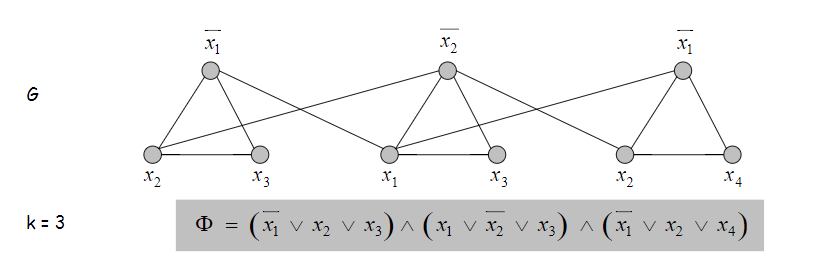
\includegraphics[width=\textwidth]{Pic/Demo}
	\end{figure}
	$\phi$ is satisfiable iff $G$ contains independent set of size $k = |\phi|$
	\begin{proof} $\Rightarrow$
	Given an assignment, select one from each triangle. This is an independent set of size k.
	\end{proof}
	\begin{proof} $\Leftarrow$
	Let $S$ be independent set of size $k$, $S$ must contain exactly one vertex in each triangle, set them to be true and the clause is still satisfied.
	\end{proof}
	Such reduction allows the conclusion that BAGEL is NP-Hard.
\end{document}
